\scanpage{45}
\diagram{\begin{tikzcd}[column sep=small,row sep=large]
U_0\arrow[r,phantom,"\subset"]&U_1\arrow[r,phantom,"\subset"]\arrow[dl,-{Hooks[harpoon]}]&U_2\arrow[d,-{Hooks[harpoon]}]&&U_3\arrow[d,-{Hooks[harpoon]}]\\
U_1^\circ\ \unsure{\subset}\arrow[d,-{Hooks[harpoon]}]&&U_2^\circ\arrow[d,-{Hooks[harpoon]}]&&U_3^\circ\arrow[d,-{Hooks[harpoon]}]\\
\partial U_1^\circ=U'_0\arrow[uu,bend left=30]&&\partial U_2^\circ\arrow[dl,-{Hooks[harpoon]}]\arrow[dr,-{Hooks[harpoon]}]&&\partial U_3^\circ\arrow[d,-{Hooks[harpoon]}]\\
&U_1^{\circ\prime}\arrow[uul,bend right=20]\arrow[dr,-{Hooks[harpoon]}]&&U''_0\arrow[uuulll,bend right=45]\arrow[dl,-{Hooks[harpoon]}]&U_2^{\circ\prime}\arrow[uull,bend right=20]\arrow[d,-{Hooks[harpoon]}]\\
&&\partial U_1^{\circ\prime}=\partial U''\arrow[uull,bend left=25]&&\partial U_2^{\circ\prime}\arrow[uull,bend right=15]
\end{tikzcd}}

\diagram{\begin{tikzcd}[column sep=small,row sep=small]
&U_n\arrow[d]&&\\
&U_n^\circ\arrow[d,-{Hooks[harpoon]}]&&\\
&\partial U_n^\circ\arrow[dl,-{Hooks[harpoon]}]\arrow[d,-{Hooks[harpoon]}]\arrow[drr,bend left=15,-{Hooks[harpoon]}]&&\\
\partial_{n-1}U_n^\circ\arrow[d]&\partial_{n-2}U_n^\circ\arrow[d]&\cdots&\partial_0U_n^\circ\arrow[d,-{Hooks[harpoon]}]\\
U_{n-1}^\circ&U_{n-2}^\circ&&U_0^\circ=U_0
\end{tikzcd}}

\figure{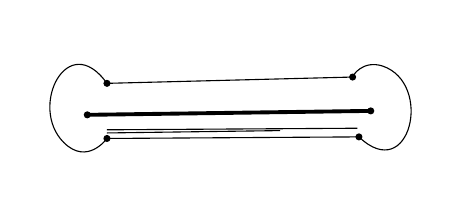
\begin{tikzpicture}[x=1cm,y=1cm]
\draw (0,.4)..controls(-.5,1.1)and(-1,.1)..(-.55,-.35)..controls(-.25,-.65)and(0,-.3)..(0,-.3)--(3.2,-.28)..controls(3.85,-.9)and(4.15,.4)..(3.5,.62)..controls(3.25,.7)and(3.12,.5)..(3.12,.48)--(0,.4);
\draw[line width=1.4pt] (-.25,0)--(3.35,.05);\draw (0,-.19)--(3.18,-.17);\draw (0,-.23)--(2.2,-.2);
\foreach \p in {(-.25,0),(0,.4),(0,-.3),(3.35,.05),(3.12,.48),(3.2,-.28)}{\fill \p circle(.045);}
\end{tikzpicture}}

\figure{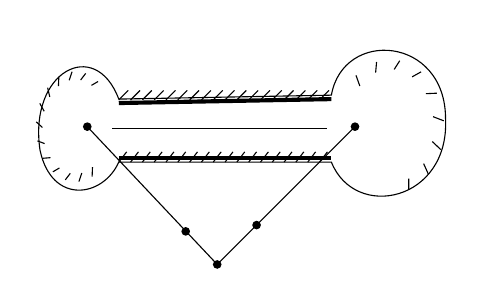
\begin{tikzpicture}[x=1cm,y=1cm]
\draw (0,.45)..controls(-.3,1.25)and(-1.15,.8)..(-1,-.2)..controls(-.85,-.9)and(-.2,-.8)..(0,-.35)--(2.7,-.35)..controls(3,-1.1)and(4.2,-.85)..(4.15,.2)..controls(4.15,1.25)and(2.85,1.35)..(2.7,.5)--(0,.45);
\draw[line width=1.5pt] (0,.4)--(2.7,.45);\draw[line width=1.5pt] (0,-.3)--(2.7,-.3);\draw (-.08,.08)--(2.65,.08);
\foreach \x in {0,.15,...,2.65}{\draw (\x,.44)--(\x+.12,.56);\draw (\x,-.35)--(\x+.1,-.22);}
\foreach \a in {55,75,...,300}{\draw ({-.55+.5*cos(\a)},{.1+.7*sin(\a)})--({-.55+.42*cos(\a+6)},{.1+.6*sin(\a+6)});}
\foreach \a in {-70,-45,...,140}{\draw ({3.45+.68*cos(\a)},{.1+.85*sin(\a)})--({3.45+.55*cos(\a+5)},{.1+.73*sin(\a+5)});}
\draw (-.4,.1)--(1.25,-1.65)--(3,.1);
\foreach \p in {(-.4,.1),(.85,-1.23),(1.25,-1.65),(1.75,-1.15),(3,.1)}{\fill \p circle(.055);}
\end{tikzpicture}}

\figure{
\begin{tikzpicture}\fill (0,0)..controls(.15,.5)and(.65,1)..(.9,1.05)--(1.15,.92)--(1.16,.72)--(1.24,.6)--(.88,.3)--(.48,-.25)--(.25,-.12)--cycle;\end{tikzpicture}}

\figure{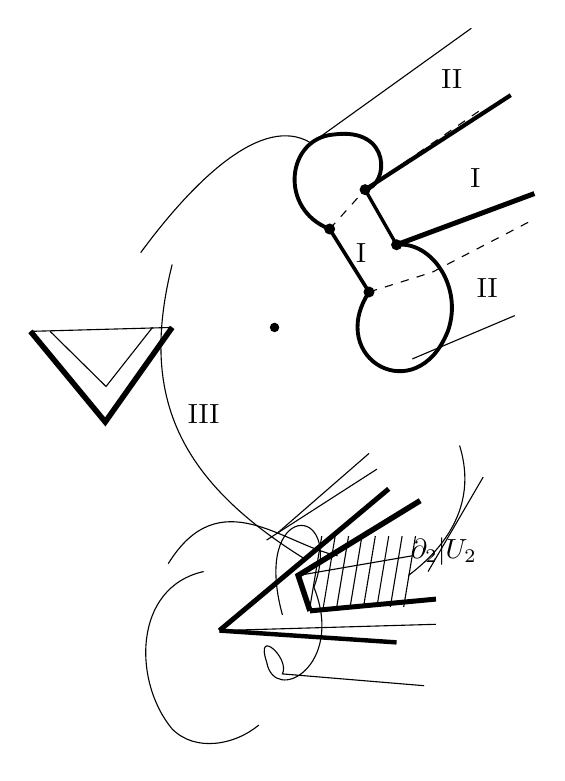
\begin{tikzpicture}[x=1cm,y=1cm]
\draw[line width=1.4pt] (3.8,4.45)..controls(3.15,4.7)and(3.25,5.6)..(3.85,5.65)..controls(4.6,5.75)and(4.55,5)..(4.25,4.95);
\draw[line width=1.3pt] (3.8,4.45)--(4.3,3.65);\draw[line width=1.2pt] (4.25,4.95)--(4.65,4.25);
\draw[line width=1.4pt] (4.3,3.65)..controls(3.75,2.8)and(4.9,2.15)..(5.3,3.15)..controls(5.5,3.7)and(5.1,4.3)..(4.65,4.25);
\draw (3.65,5.6)--(5.6,7);\draw[line width=1.5pt] (4.25,4.95)--(6.1,6.15);\draw[line width=1.8pt] (4.65,4.25)--(6.4,4.9);\draw (4.85,2.8)--(6.15,3.35);
\draw[dashed] (3.8,4.45)--(4.25,4.95)--(5.7,5.95);\draw[dashed] (4.3,3.65)--(5.1,3.9)--(6.35,4.55);
\foreach \p in {(3.8,4.45),(4.25,4.95),(4.3,3.65),(4.65,4.25)}{\fill \p circle(.07);}
\node at (5.35,6.35) {$\mathrm{II}$};\node at (5.65,5.1) {$\mathrm I$};\node at (4.2,4.15) {$\mathrm I$};\node at (5.8,3.7) {$\mathrm{II}$};
\fill (3.1,3.2) circle(.06);
\draw (1.4,4.15)..controls(2.1,5.1)and(2.95,5.9)..(3.55,5.55);
\draw (0,3.15)--(1.8,3.2);\draw[line width=2pt] (0,3.15)--(.95,2)--(1.8,3.2);\draw (.25,3.15)--(.96,2.45)--(1.55,3.2);
\draw (1.8,4)..controls(1.4,2.4)and(1.8,1.3)..(3.5,.25);\node at (2.2,2.1) {$\mathrm{III}$};
\draw (2.2,.1)..controls(1.3,-.1)and(1.3,-1.3)..(1.8,-1.9)..controls(2.1,-2.2)and(2.6,-2.1)..(2.9,-1.85);
\draw (1.75,.2)..controls(2.4,1.25)and(3.2,.45)..(3.9,.3);
\draw[line width=1.8pt] (2.4,-.65)--(4.55,1.15);\draw[line width=1.6pt] (2.4,-.65)--(4.65,-.8);
\draw[line width=2pt] (3.55,-.4)--(3.4,.05)--(4.95,1);\draw[line width=1.8pt] (3.55,-.4)--(5.15,-.25);
\draw (2.4,-.65)--(5.15,-.57);\draw (3.4,.05)--(4.85,.3);\draw (3,.5)--(4.4,1.4);\draw (3.15,.6)--(4.3,1.6);
\foreach \x in {3.55,3.72,...,4.75}{\draw (\x,-.35)--(\x+.15,.55);}
\draw (3.2,-.45)..controls(2.8,1)and(4,1)..(3.6,-.1)..controls(4,-1.1)and(3.1,-1.6)..(3,-1.05)..controls(2.85,-.6)and(3.3,-1)..(3.2,-1.2)--(5,-1.35);
\draw (4.8,.05)..controls(5.2,.35)and(5.7,.9)..(5.45,1.7);\draw (5.05,.1)--(5.75,1.3);
\node at (5.25,.35) {$\deleted{\unsure{\partial_2|U_2}}$};
\end{tikzpicture}}
% crop-candidate: scan 45

\figure{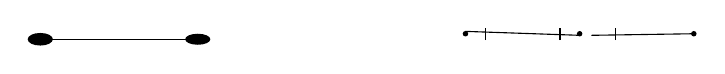
\begin{tikzpicture}[x=1cm,y=1cm]
\draw (0,0)--(2,0);\fill (0,0) ellipse(.16 and .08);\fill (2,0) ellipse(.16 and .07);
\draw (5.4,.1)--(6.85,.05);\draw (7,.05)--(8.3,.07);\foreach \x in {5.65,6.6,7.3}{\draw (\x,-.01)--(\x,.14);}\foreach \x in {5.4,6.85,8.3}{\fill (\x,.07) circle(.035);}
\end{tikzpicture}}

\figure{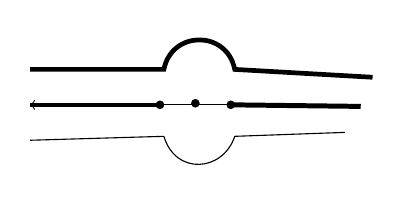
\begin{tikzpicture}[x=1cm,y=1cm]
\draw[line width=1.7pt] (0,.45)--(1.7,.45)..controls(1.8,.95)and(2.5,.95)..(2.6,.45)--(4.35,.35);
\draw[line width=1.3pt] (0,0)--(1.65,0);\draw (1.65,0)--(2.55,0);\draw[line width=1.8pt] (2.55,0)--(4.2,-.02);
\draw[<-] (0,0)--(.5,0);
\draw (0,-.45)--(1.7,-.4)..controls(1.85,-.9)and(2.45,-.85)..(2.6,-.4)--(4,-.35);
\foreach \p in {(1.65,0),(2.1,.02),(2.55,0)}{\fill \p circle(.055);}
\end{tikzpicture}}

\figure{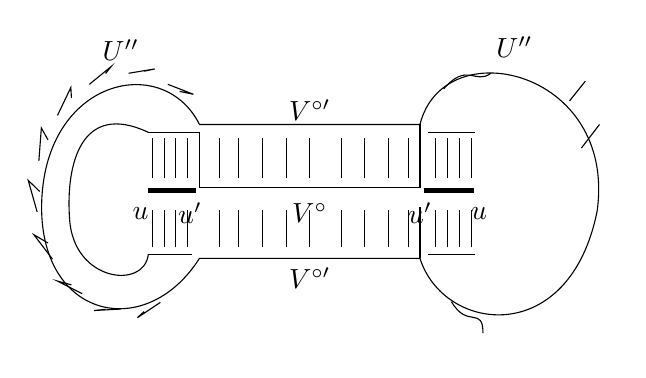
\begin{tikzpicture}[x=1cm,y=1cm]
\draw (0,1)..controls(-.45,1.9)and(-1.9,1.6)..(-2,.1)..controls(-2.1,-1.45)and(-.7,-1.8)..(0,-.7)--(2.8,-.7)..controls(3.1,-1.65)and(4.7,-1.85)..(5.05,-.1)..controls(5.3,1.7)and(3.1,2.2)..(2.8,1)--(0,1);
\draw (-.65,.9)..controls(-1.5,1.3)and(-1.7,.5)..(-1.65,-.2)..controls(-1.6,-1)and(-.7,-1.1)..(-.65,-.65);
\draw (-.65,.9)--(0,.9)--(0,.2)--(2.8,.2)--(2.8,1);\draw (-.65,-.65)--(-.1,-.65);\draw (2.8,-.7)--(2.8,-.05);
\draw[line width=1.8pt] (-.65,.16)--(-.05,.16);\draw[line width=1.8pt] (2.85,.16)--(3.48,.16);
\draw (2.9,.9)--(3.5,.9);\draw (2.9,-.65)--(3.5,-.65);
\foreach \x in {-.6,-.45,-.3,-.15,.25,.5,.8,1.1,1.4,1.8,2.1,2.4,2.65,3,3.15,3.3,3.45}{\draw (\x,.32)--(\x,.83);\draw (\x,-.56)--(\x,-.08);}
\foreach \a in {55,80,...,290}{\draw ({-.9+1.13*cos(\a)},{.15+1.55*sin(\a)})--({-.9+1.28*cos(\a-5)},{.15+1.61*sin(\a-5)})--({-.9+1.18*cos(\a+10)},{.15+1.5*sin(\a+10)});}
\draw (3.1,1.45)..controls(3.4,1.8)and(3.5,1.5)..(3.7,1.65);\draw (4.7,1.3)--(4.9,1.55);\draw (4.85,.7)--(5.08,1);\draw (3.2,-1.25)..controls(3.4,-1.6)and(3.6,-1.3)..(3.6,-1.65);
\node at (-1,1.95) {$U''$};\node at (4,1.98) {$U''$};\node at (1.4,1.18) {$V^{\circ\prime}$};\node at (1.4,-.95) {$V^{\circ\prime}$};\node at (1.4,-.12) {$V^\circ$};
\node at (-.75,-.13) {$u$};\node at (-.12,-.13) {$u'$};\node at (2.8,-.13) {$u'$};\node at (3.55,-.13) {$u$};
\end{tikzpicture}}

\figure{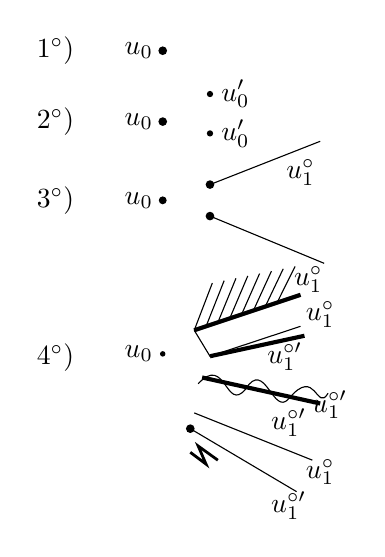
\begin{tikzpicture}[x=1cm,y=1cm]
\node[anchor=east] at (-1,8.8) {$1^\circ)$};\node[left] at (0,8.8) {$u_0$};\fill (0,8.8) circle(.055);
\node[anchor=east] at (-1,7.9) {$2^\circ)$};\node[left] at (0,7.9) {$u_0$};\fill (0,7.9) circle(.055);
\fill (.6,8.25) circle(.04);\node[right] at (.62,8.25) {$u'_0$};\fill (.6,7.75) circle(.04);\node[right] at (.62,7.75) {$u'_0$};
\node[anchor=east] at (-1,6.9) {$3^\circ)$};\node[left] at (0,6.9) {$u_0$};\fill (0,6.9) circle(.05);
\draw (.6,7.1)--(2,7.65);\draw (.6,6.7)--(2.05,6.1);\fill (.6,7.1) circle(.055);\fill (.6,6.7) circle(.055);\node at (1.75,7.25) {$u_1^\circ$};\node at (1.85,5.9) {$u_1^\circ$};
\node[anchor=east] at (-1,4.9) {$4^\circ)$};\node[left] at (0,4.95) {$u_0$};\fill (0,4.95) circle(.035);
\draw[line width=1.5pt] (.4,5.25)--(1.75,5.7);\draw (.4,5.25)--(.6,4.92)--(1.75,5.3);\draw[line width=1.5pt] (.6,4.92)--(1.8,5.18);
\foreach \x in {.4,.55,...,1.6}{\draw (\x,{5.25+(\x-.4)*.33})--({\x+.23},{5.85+(\x-.4)*.2});}
\node at (2,5.45) {$u_1^\circ$};\node at (1.55,4.92) {$u_1^{\circ\prime}$};
\draw[line width=1.5pt] (.5,4.65)--(2,4.32);\draw (.45,4.57)..controls(.8,4.95)and(.8,4.2)..(1.05,4.5)..controls(1.3,4.9)and(1.4,4.15)..(1.6,4.38)..controls(1.95,4.8)and(1.95,4.2)..(2.1,4.45);
\node at (2.12,4.3) {$\deleted{\unsure{u_1^{\circ\prime}}}$};
\draw (.4,4.2)--(1.9,3.6);\draw (.35,4.0)--(1.7,3.2);\fill (.35,4) circle(.055);\draw[line width=1pt] (.35,3.7)--(.55,3.55)--(.45,3.78)--(.7,3.6);
\node at (1.6,4.08) {$u_1^{\circ\prime}$};\node at (2,3.45) {$u_1^\circ$};\node at (1.6,3.02) {$u_1^{\circ\prime}$};
\end{tikzpicture}}

\figure{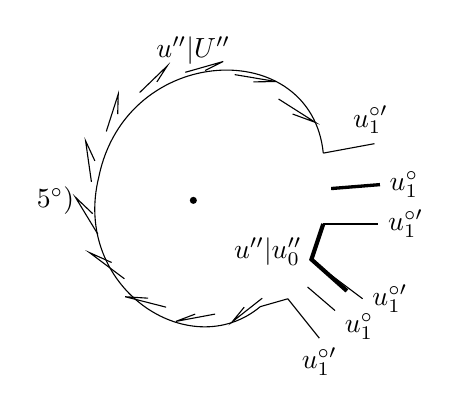
\begin{tikzpicture}[x=1cm,y=1cm]
\node at (-2.4,1) {$5^\circ)$};\fill (-.65,1) circle(.045);
\draw (1,1.6)..controls(.85,3.1)and(-1.5,3)..(-1.85,1.3)..controls(-2.2,-.1)and(-.7,-1.1)..(.2,-.35)--(.55,-.25);
\draw (1,1.6)--(1.65,1.72);\draw[line width=1.2pt] (1.1,1.15)--(1.72,1.2);\draw (1,.7)--(1.7,.7);\draw[line width=1.5pt] (1,.7)--(.85,.25)--(1.3,-.15);
\draw (.55,-.25)--(.95,-.75);\draw (.8,-.1)--(1.15,-.4);\draw (1.1,.05)--(1.5,-.25);
\foreach \a in {40,65,...,290}{\draw ({-.5+1.45*cos(\a)},{1.1+1.55*sin(\a)})--({-.5+1.65*cos(\a-8)},{1.1+1.68*sin(\a-8)})--({-.5+1.45*cos(\a+10)},{1.1+1.55*sin(\a+10)});}
\node at (-.65,2.9) {$\unsure{u''|U''}$};\node[above] at (1.6,1.72) {$u_1^{\circ\prime}$};\node[right] at (1.72,1.2) {$u_1^\circ$};\node[right] at (1.7,.7) {$u_1^{\circ\prime}$};\node[left] at (.85,.35) {$\unsure{u''|u_0''}$};
\node[right] at (1.5,-.25) {$u_1^{\circ\prime}$};\node[right] at (1.15,-.6) {$u_1^\circ$};\node[below] at (.95,-.75) {$u_1^{\circ\prime}$};
\end{tikzpicture}}

\figure{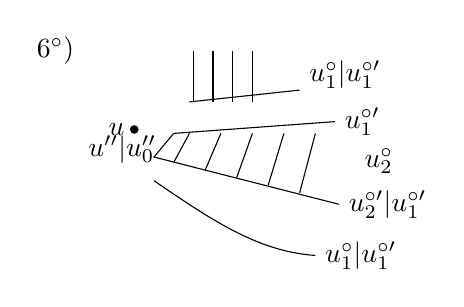
\begin{tikzpicture}[x=1cm,y=1cm]
\node at (-1.8,1.3) {$6^\circ)$};\node[left] at (-.8,.3) {$u$};\fill (-.8,.3) circle(.055);
\draw (-.1,.65)--(1.3,.8);\foreach \x in {-.05,.2,.45,.7}{\draw (\x,.65)--(\x,1.3);}\node[right] at (1.3,1) {$\unsure{u_1^\circ|u_1^{\circ\prime}}$};
\draw (-.3,.25)--(1.75,.4);\draw (-.3,.25)--(-.55,-.05)--(1.8,-.65);\foreach \x in {-.3,.1,.5,.9,1.3}{\draw (\x,{-.12-(\x+.3)*.24})--({\x+.2},.25);}
\draw (-.55,-.35)..controls(.25,-.9)and(.8,-1.25)..(1.5,-1.3);
\node[right] at (1.75,.4) {$u_1^{\circ\prime}$};\node[right] at (2,-.1) {$u_2^\circ$};\node[right] at (1.8,-.65) {$\unsure{u_2^{\circ\prime}|u_1^{\circ\prime}}$};\node[right] at (1.5,-1.3) {$\unsure{u_1^\circ|u_1^{\circ\prime}}$};\node[left] at (-.4,.05) {$\unsure{u''|u_0''}$};
\end{tikzpicture}}
\mspage{46}
